% Chapter 1
\setchapterimage{jet}
\setchapterpreamble[u]{\margintoc}
\chapter{Fusion: general introduction}\label{Chapter1}
% For referencing the chapter elsewhere, use \ref{Chapter1} 

blablabla need for clean and abundant energy

\section{Thermonuclear fusion}
\begin{itemize}
    \item e=mc2
    \item DT reaction
    \item magnetic confinement --> Tokamak
    \item triple product
    \item Choice of a plasma facing material
\end{itemize}

The fundamental principle of nuclear fusion is to fuse two light nuclei into a heavier nucleus.
The mass difference between the products and the reactants is released in the form of energy (see Equation \ref{eq: emc2}).
\begin{equation}
    E = \Delta m c^2
    \label{eq: emc2}
\end{equation}
where $\Delta m$ is the mass difference, $c$ is the speed of light.
This process is the opposite process of nuclear fission, powering the current nuclear plants.

When looking at the different binding energies per nucleon of the elements (see Figure \ref{fig: binding energy per nucleon}), it becomes clear that light elements release energy from fusion and heavy elements release energy from fission.

\begin{figure} [h]
    \centering
    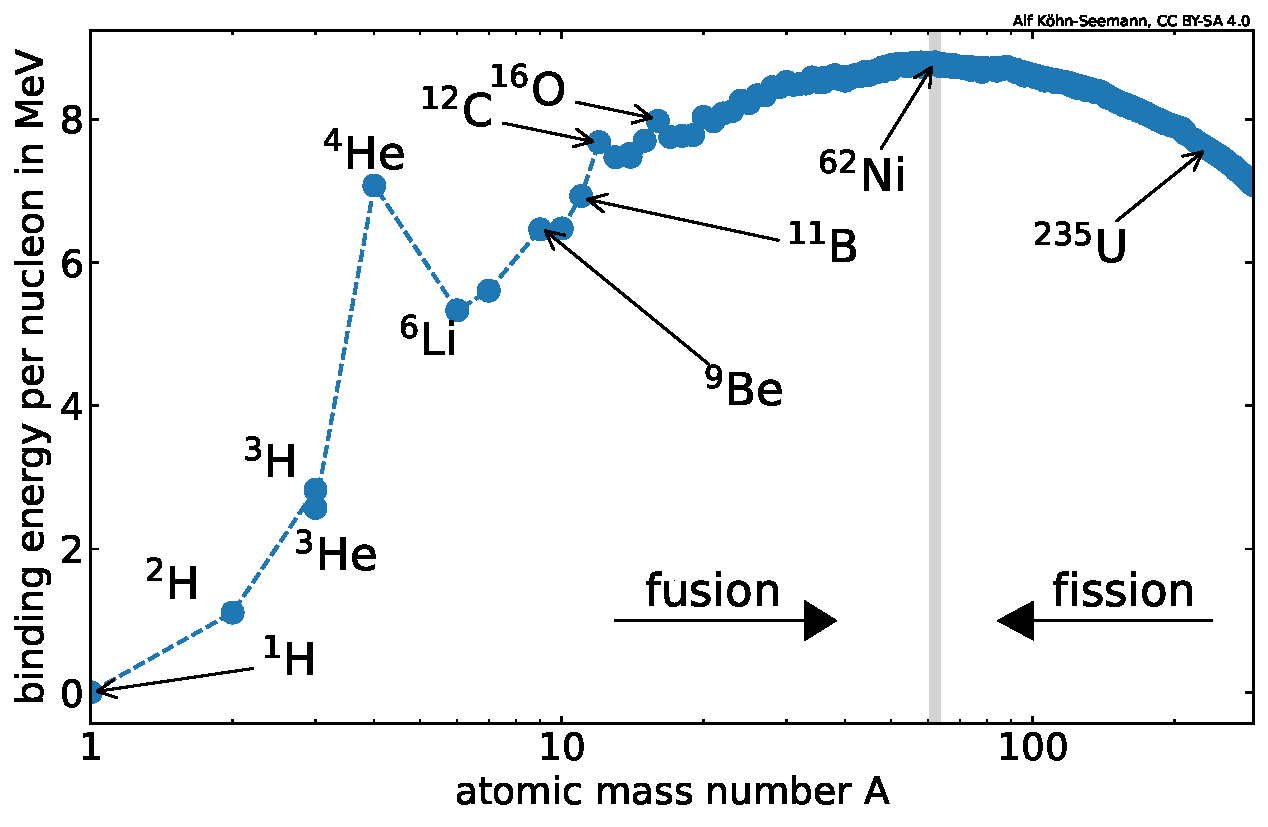
\includegraphics[width=\linewidth]{Figures/Chapter1/binding_energy_per_nucleon.pdf}
    \caption{Binding energy per nucleon \cite{kohn-seemann_alfkoehnfusion_plots_2021}}
    \label{fig: binding energy per nucleon}
\end{figure}

Nuclei are positively charged.
To be able to fuse, these must overcome the Coulomb barrier induced by the electromagnetic repulsion (see Figure \ref{fig: potential energy diagram fusion}).
This Coulomb barrier increases with the charge of the nuclei (\textit{ie} the number of protons).
This means that the nuclei must collide with a high enough velocity.
At the atomistic scale, the velocity $v_\mathrm{th}$ is a function of temperature (see Equation \ref{eq: thermal velocity}).
This is one of the reasons why the probability of a fusion reaction (called cross-section) is temperature dependent.

\begin{equation}
    v_\mathrm{th} = \sqrt{\frac{k_B T}{m}}
    \label{eq: thermal velocity}
\end{equation}
where $k_B = \SI{1.3806e-23}{m^2.s^{-2}.kg.K^{-1}}$ is the Boltzmann constant, $T$ is the nucleus temperature in \si{K} and $m$ is the nucleus mass in \si{kg}.


\begin{figure} [h]
    \centering
    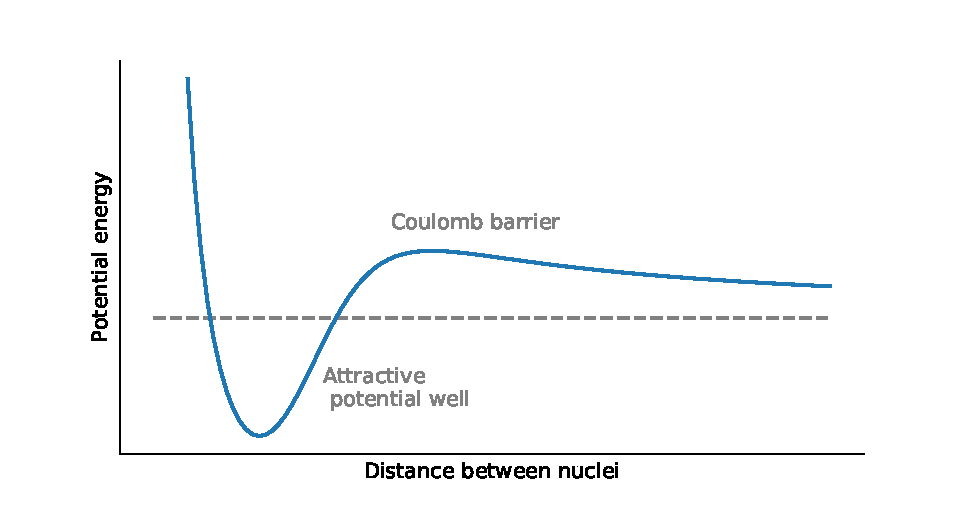
\includegraphics[width=\linewidth]{Figures/Chapter1/potential_energy.pdf}
    \caption{Potential energy diagram}
    \label{fig: potential energy diagram fusion}
\end{figure}

Hydrogen, as the lightest element, has the lowest fusion temperature.
It is also the most abundant element on Earth (although bond to other elements).
Depending on which hydrogen isotope is used, different fusion reactions are available (see Equations \ref{eq: fusion reactions}).
Each of these reactions has a different cross-section.

\begin{subequations}
    \begin{equation}
         \ce{^2H + ^2H -> ^3H (\SI{1.01}{MeV})+ n (\SI{3.02}{MeV})}
    \end{equation}
    \begin{equation}
        \ce{^2H + ^2H -> ^3He (\SI{0.82}{MeV}) + n (\SI{2.45}{MeV})}
    \end{equation}
    \begin{equation}
        \ce{^2H + ^3H -> ^4He (\SI{3.5}{MeV}) + n (\SI{14.1}{MeV})}
    \end{equation}
    \begin{equation}
        \ce{^2H + ^3He -> ^4He (\SI{3.6}{MeV}) + p (\SI{14.7}{MeV})}
    \end{equation}
    \label{eq: fusion reactions}
\end{subequations}

\begin{figure} [h]
    \centering
    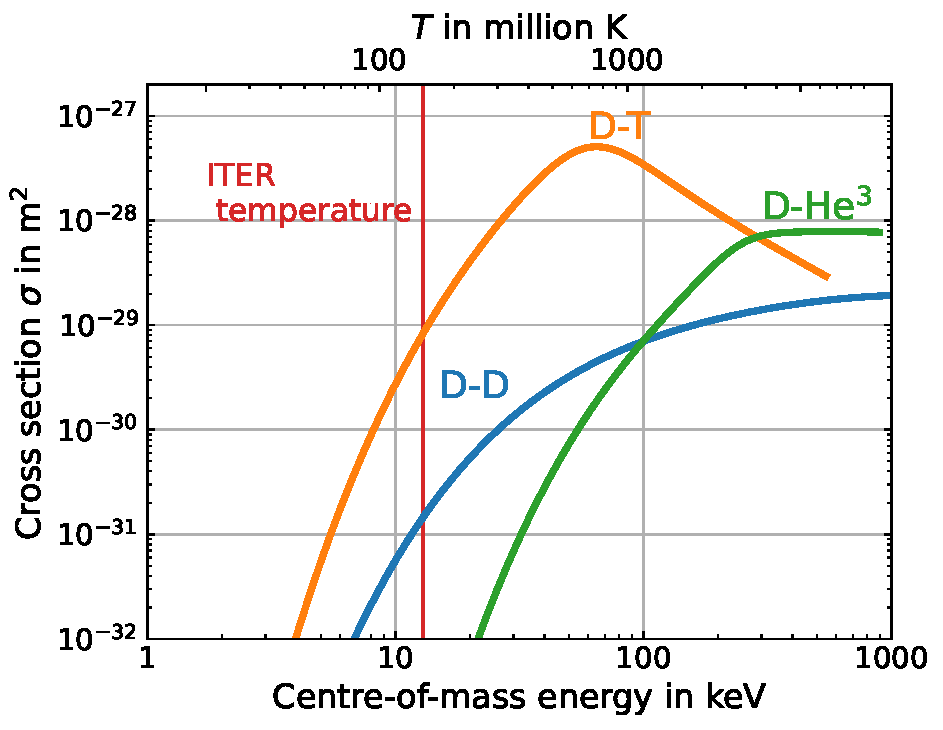
\includegraphics[width=\linewidth]{Figures/Chapter1/cross_sections_vs_temperature__Bosch.pdf}
    \caption{Fusion cross sections}
    \label{fig: fusion cross sections}
\end{figure}

The deuterium-tritium (DT) reaction is the one with the highest cross-section (probability) at "low" temperature (see Figure \ref{fig: fusion cross sections}).
This is the reason why this reaction has been the focus of nuclear fusion for decades.
More recently, private companies have started experimenting with more exotic reactions like proton-boron (TAE Technologies) or D-He3 (Helion Energy).

% \begin{figure} [h]
%     \centering
%     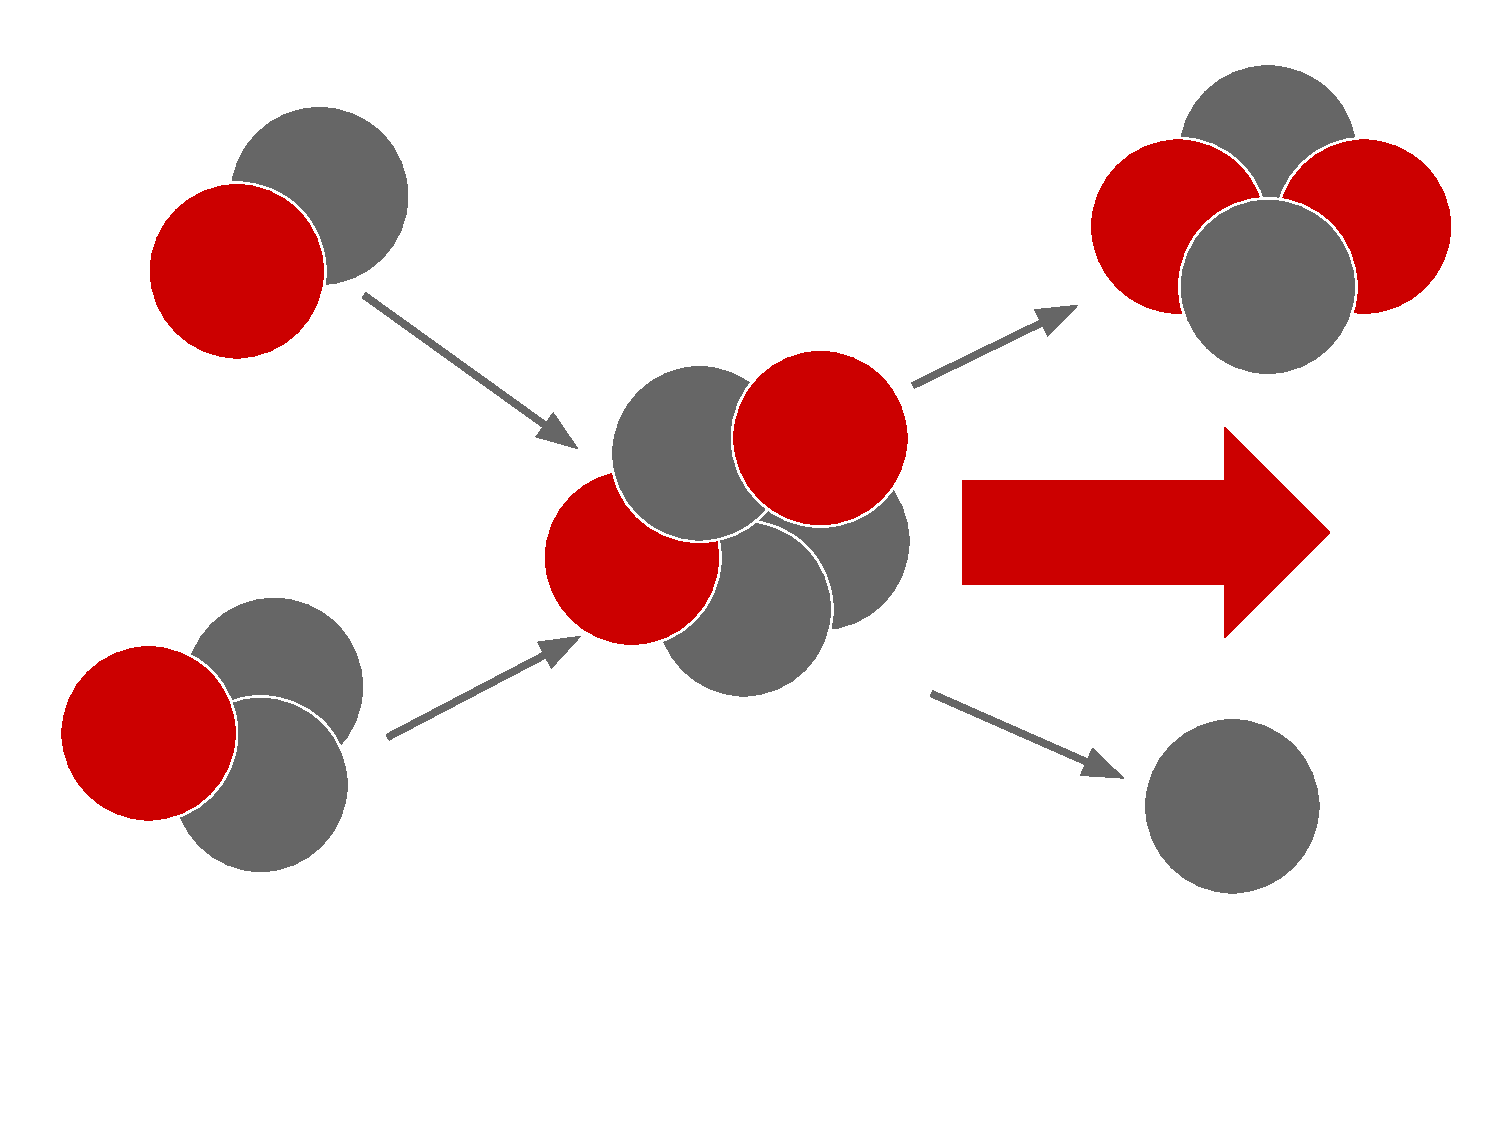
\includegraphics[width=\linewidth]{Figures/Chapter1/nuc_fus.pdf}
%     \caption{DT reaction}
% \end{figure}

\section{Tokamaks: how to bottle a star}

\subsection{Technology}
As explained above, for fusion to occur, the fuel must be heated up to millions of degrees.
A these temperatures, the DT gas becomes a plasma where electrons are teared out from the nuclei.
The principle of magnetic confinement reactors is to trap the electrically charged particles in a magnetic cage.
The electrons and ions then gyrate around the magnetic field lines and the Larmor radius of the gyration is given by:
\begin{equation}
    R =  \frac{\sqrt{2 m T}}{e B}
\end{equation}
where $m$ is the mass of the particle, $T$ its temperature, $e$ its charge and $B$ the magnetic field.
In a hot plasma (\SI{10}{keV}) with a strong magnetic field of \SI{3}{T}, the Larmor radius of ions is $\approx \SI{1}{mm}$, which is much smaller compared to the size of a reactor.
The Larmor radius of an electron is orders of magnitude smaller due to its lower mass.
Straight magnetic lines can therefore confine charged particles in the direction perpendicular to the field lines.
However, the particles are not confined in the parrallel direction.

This issue can be solved by closing the field lines, forming a torus-shaped magnetic field.
However, this configuration poses another problem: bending the field lines creates a magnetic field gradient in the radial direction.
This magnetic field gradient and the centrifugal force cause the particles to drift upwards (or downwards depending on their charge).
Due to this drift, the particles end up escaping the magnetic confinement until they touch the walls of the chamber and neutralise (making it impossible for them to fuse).

Two options exist to compensate this drift.
The first is to add a poloidal component to the magnetic field and twist the magnetic lines.
This is done by inducting a current in the plasma thanks to a central solenoïd (see Figure~\ref{fig:tokamak magnetic field}).
This configuration is called Tokamak which stands for "toroidalnaïa kamera s magnitnymi katouchkami" (toroidal chamber with magnetic coils).

\begin{figure}[h]
    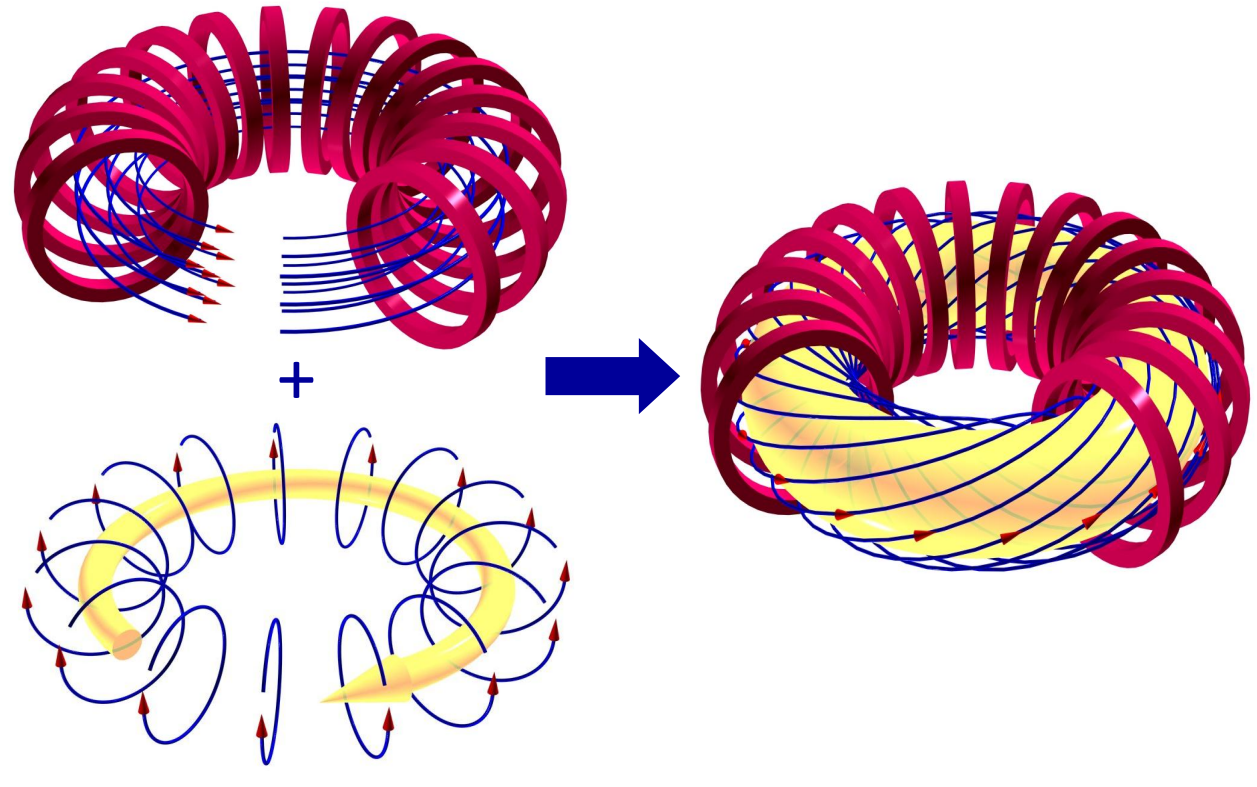
\includegraphics[width=\linewidth]{Figures/Chapter1/tokamak_magnetic_fields.png}
    \caption{Magnetic field lines in a tokamak. Contribution of the toroidal and poloidal components.}
    \label{fig:tokamak magnetic field}
\end{figure}

The second option is to twist the magnetic field by twisting the toroidal coils themselves.
This configuration is called a stellarator and has the advantage of not having an induced current and is therefore inherently steady-state.
The tokamak, on the other hand, is a pulsed device.
This is because the central solenoid has a limited capacity.
The main drawback of the the stellarator is the complexity of the coils.
Since each coil has a unique shape, the cost of manufacturing such a reactor is higher than tokamaks for which coils can be manufactured in serial.

\subsection{Triple product}
The power balance in a fusion reactor is given by:
\begin{equation}
    \frac{\partial W}{\partial t} = P_\mathrm{fusion} + P_\mathrm{heating} - P_\mathrm{losses}
    \label{eq: plasma energy balance}
\end{equation}
$W$ is the thermal energy stored in the plasma and can be expressed in \si{J.m^{-3}} by:
\begin{equation}
    W = 3 n T
\end{equation}
where $n$ is the plasma density in \si{m^{-3}} and $T$ is the plasma temperature in \si{eV}.
$P_\mathrm{fusion}$, expressed in \si{W.m^{-3}}, is the power generated from fusion reactions themselves and can be expressed by:
\begin{equation}
    P_\mathrm{fusion} = n_D n_T \left\langle \sigma \right\rangle E
\end{equation}
where $n_D$ and $n_T$ are the densities in \si{m^{-3}} of deuterium and tritium respectively, $\left\langle \sigma \right\rangle$ is the DT cross-section in \si{m^3.s^{-1}} and $E$ is the energy of the fusion reaction in \si{J}.
Because the neutrons have little interaction with the plasma, $E \approx E_\alpha = \SI{3.56}{MeV}$.
Moreover, assuming a 50\%-50\% mixture of deuterieum and tritium, $n_D = n_T = \frac{1}{2} n$.
The fusion power can therefore be written as:
\begin{equation}
    P_\mathrm{fusion} = \frac{1}{4} n^2 \left\langle \sigma \right\rangle E_\alpha
\end{equation}

The amplification factor $Q$ defines the ratio of the fusion power by the heating power.
The heating power $P_\mathrm{heating}$ is therefore written as:
\begin{equation}
    P_\mathrm{heating} = \frac{P_\mathrm{fusion}}{Q}
\end{equation}

Finally, $P_\mathrm{losses}$ is the rate at which the plasma loses energy, either by losing mass (particles escaping the magnetic cage) or by radiation.
It is characterised by an energy confinement time $\tau_E$ and can be expressed as:
\begin{equation}
    P_\mathrm{losses} = \frac{W}{\tau_E} = \frac{3 n T}{\tau_E}
\end{equation}

Assuming energy equilibrium (\textit{ie} $\frac{\partial W}{\partial t} = 0$) Equation \ref{eq: plasma energy balance} can therefore be written as:
\begin{align}
    P_\mathrm{losses} &= P_\mathrm{fusion} + P_\mathrm{heating} \\
    \Leftrightarrow \frac{3 n T}{\tau_E} &= \frac{1}{4} n^2 \left\langle \sigma \right\rangle E_\alpha + \frac{P_\mathrm{fusion}}{Q}
\end{align}

Re-arranging the terms, one can obtain:
\begin{equation}
    n T \tau_E = \frac{12 T^2}{\left\langle \sigma \right\rangle E_\alpha} \cdot \frac{1}{1 + \frac{1}{Q}}
    \label{eq: triple product}
\end{equation}

$n T \tau_E$ is known as the \textit{triple product}, a figure of merit describing the performance of a fusion reactor.
Equation \ref{eq: triple product} gives the triple-product required to achieve a given amplification factor $Q$ at a given temperature $T$.

When $P_\mathrm{heating}$ approaches zero (\textit{ie} the auxilliary heating systems are shut down), the amplification factor $Q$ approaches $\infty$.
Therefore 
\begin{equation}
    n T \tau_E \rightarrow \frac{12 T^2}{\left\langle \sigma \right\rangle E_\alpha} \geq \SI{3e21}{keV.s.m^{-3}}
\end{equation}

This is known as the Lawson criterion, which needs to be satisfied in order to reach \textit{ignition} ($Q = \infty$).


Fusion devices can therefore be classified into three categories.
Stars like our Sun have very high confinement times and densities while remaining at relatively low temperatures (the sun Core is at \SI{1.2}{keV}).
Magnetic confinement devices (tokamaks, stellarators, etc.) exhibit temperatures orders of magnitude higher than stars but have confinement times of the order of $\sim \SI{1}{s}$.
A third way of achieving fusion is to heat and compress a target of fuel with either lasers (NIF, Laser Mega Joule), pistons (General Fusion) or by smashing it at high speed with a projectile (First Light Fusion).
These devices, known as \textit{inertial fusion devices}, exhibit extremely high densities ($\sim \SI{e31}{m^{-3}}$) but short confinement times ($\sim \SI{e-11}{s}$).
 
So far, no fusion device has been able to even reach \textit{break-even} ($Q = 1$) (see Figure \ref{fig: triple product vs T}).
The record of $Q = 0.68$ by the European tokamak JET (Joint European Torus) and was performed in 1997.
The objective of the ITER tokamak, currently under construction in France, is to demonstrate an amplification factor of $Q=10$ over \SI{400}{s}. 

\begin{figure}
    \centering
    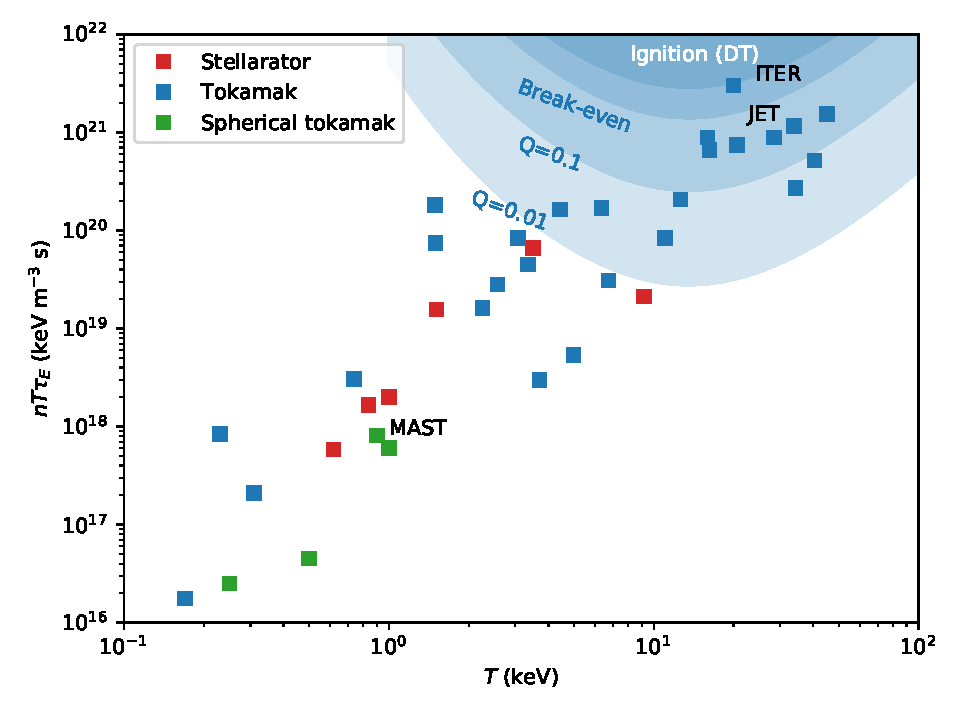
\includegraphics[width=\linewidth]{Figures/Chapter1/triple_product_vs_T.pdf}
    \caption{Triple product. An interactive version of this plot is available at \href{https://remdelaportemathurin.github.io/fusion-world/}{https://remdelaportemathurin.github.io/fusion-world/}.}
    \label{fig: triple product vs T}
\end{figure}

\subsection{Divertor}
\begin{itemize}
    \item Particle and heat exhaust
    \item Different types of divertors (double null, super x, snowflake...)
    \item Actively cooled divertors with monoblocks
\end{itemize}

\subsection{Plasma-facing materials}
\begin{itemize}
    \item checklist of a plasma facing material
    \item candidates (tungsten, berylium)
\end{itemize}

\section{Plasma-surface interactions in tokamaks}

The wall of a fusion reactor (first wall and divertor) is bombarded with high energy hydrogen (deuterium and tritium) and helium ions.
Due to their small size, these ions can penetrate the metal lattice and be implanted in the material.

Many interactions occur between hydrogen, helium and tungsten atoms.

\subsection{H/W \& He/W interactions}
\begin{figure*}[h!]
    \begin{subfigure}{0.9\linewidth}
        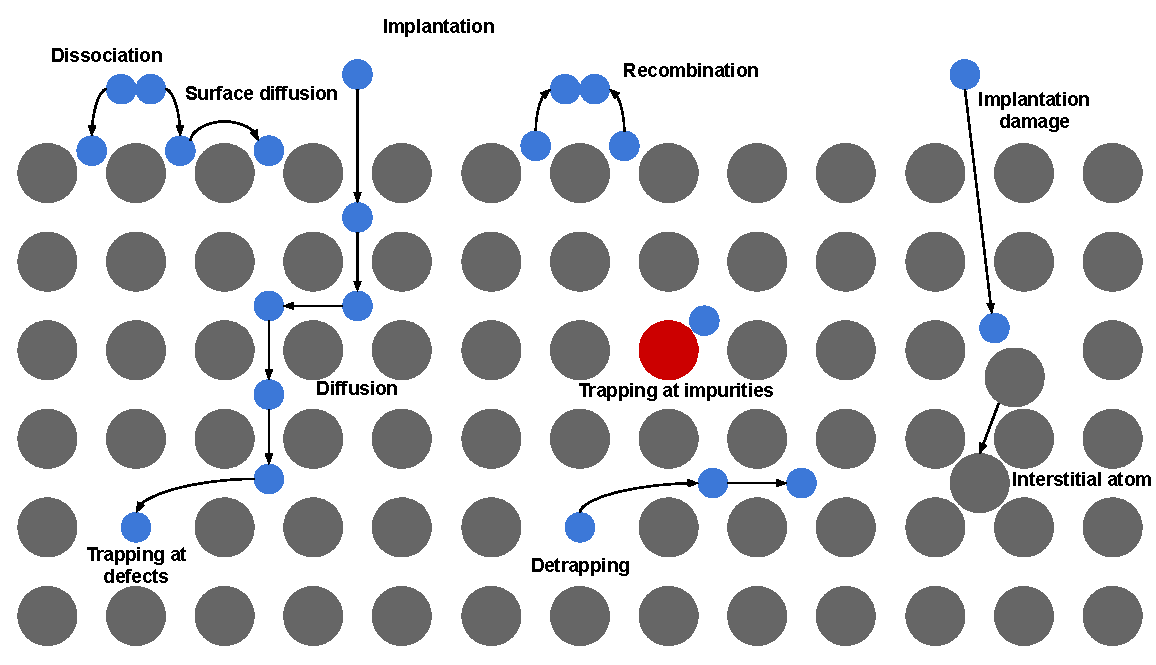
\includegraphics[width=\linewidth]{Figures/Chapter1/HI transport sketch.pdf}
        \caption{H}
    \end{subfigure}
    \begin{subfigure}{0.9\linewidth}
        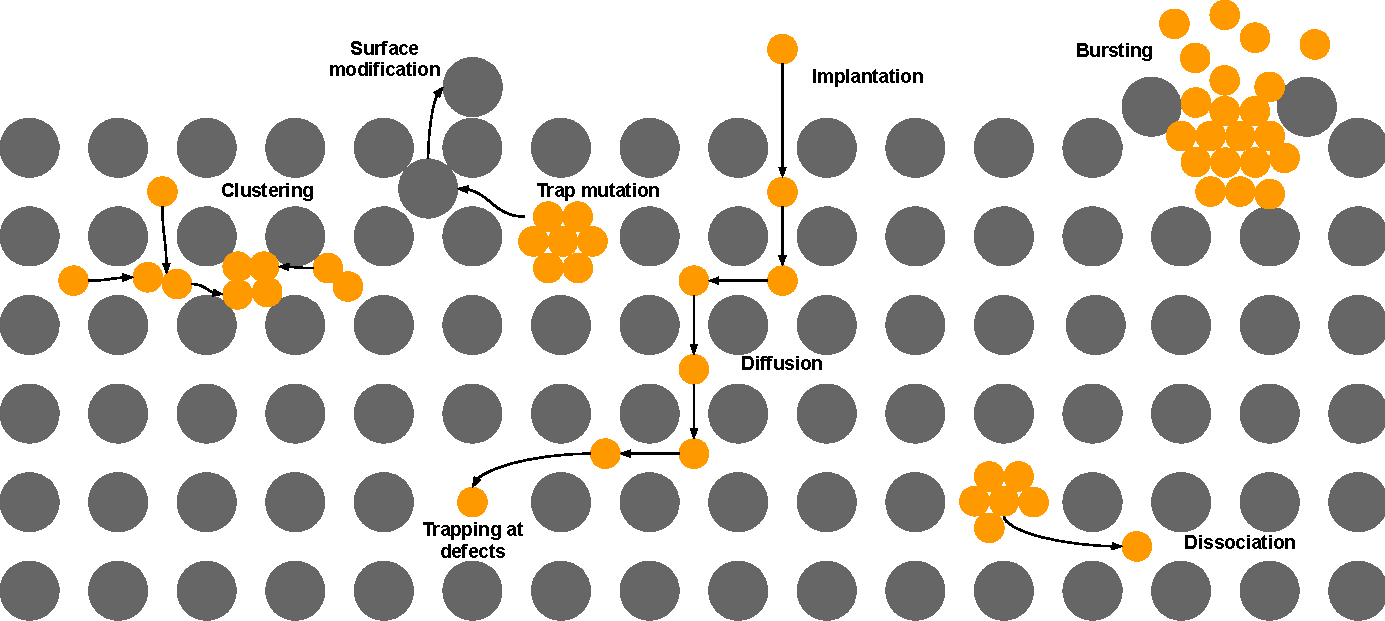
\includegraphics[width=\linewidth]{Figures/Chapter1/He transport sketch.pdf}
        \caption{He}
    \end{subfigure}
    \caption{Interactions of solute species in tungsten}
\end{figure*}

\begin{itemize}
    \item potential energy diagram
\end{itemize}

\subsubsection{Diffusion}
Diffusion of solute species is thermally activated and the diffusion coefficient $D$ expressed in \si{m^2.s^{-1}} usually follows an Arrhenius law:
\begin{equation}
    D = D_0 \exp{(-E_D/k_B T)}
\end{equation}

% MD simulations
Diffusion coefficients (also called diffusivities) can be computed by Molecular Dynamics (MD).
The principle of Molecular Dynamics is to calculate the trajectory of atoms in a simulation box.
The trajectory of a particle $i$ in a system of $N$ particles can be computed from Newton's second law of motion:

\begin{equation}
    m_i \vec{a_i} = \sum_{j=1 \, j \neq i}^N \vec{F}_{i,j}
\end{equation}
where $m_i$ is the mass of the particle, $\vec{a_i}$ is its acceleration, $\vec{F}_{i,j}$ is the force applied to the particle due to its interaction with particle $j$.
The forces between atoms is only a function of the interatomic potentials that can be estimated from \textit{ab initio} computations (Density Functional Theory) \cite{connetable_diffusion_2019,fernandez_hydrogen_2015,boisse_modelling_2014,boisse_modeling_2014,becquart_microstructural_2010} or from methods based on machine learning (pseudo-potentials) [insert refs].

By measuring the trajectory of a diffusing species from MD simulations for a long time, its diffusion coefficient $D$ can be estimated from Einstein equation \cite{einstein_uber_1905}:
\begin{equation}
    \lim_{x\to\infty} \frac{\langle R^2(t) \rangle}{6t} = D
\end{equation}
where $\langle R^2(t) \rangle$ is the mean squared displacement of the species.

This method was used to estiamte the diffusion coefficient of H in W \cite{wang_molecular_2020, zhou_molecular_2016,kato_super-saturated_2015,liu_hydrogen_2014} and for He in W \cite{faney_numerical_2013,faney_spatially_2014,faney_spatially_2015,sefta_surface_2013,perez_mobility_2017}.
\begin{figure}
    \centering
    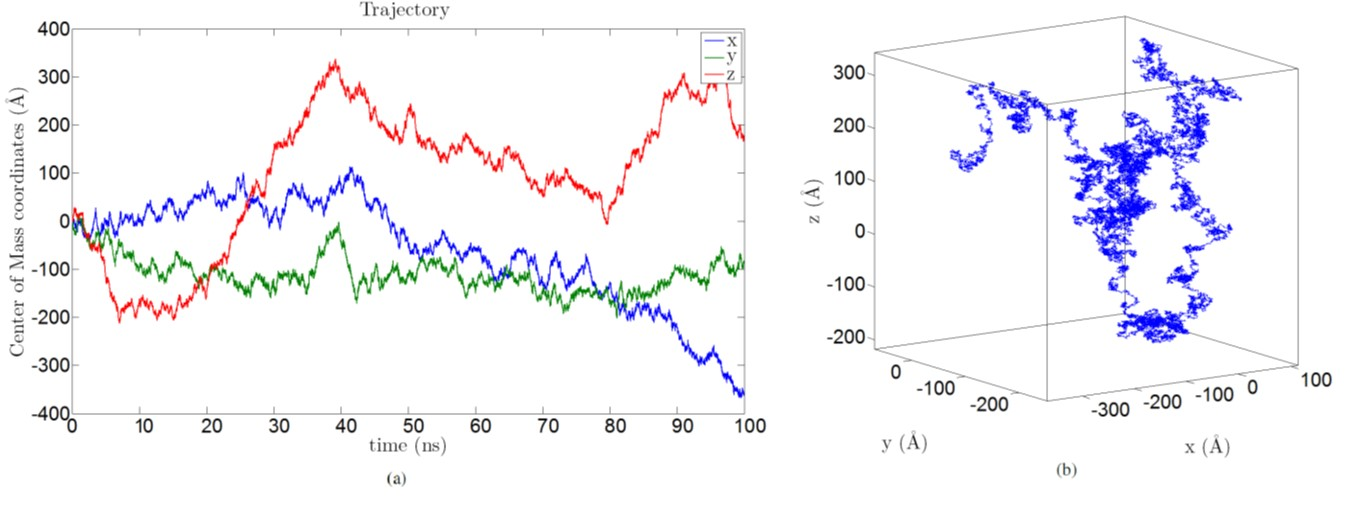
\includegraphics[width=0.7\linewidth]{Figures/Chapter1/faney_md.jpg}
    \caption{Example of the trajectory of a He$_2$ cluster. Reproduced from \cite{faney_numerical_2013}}
    \label{fig: md faney}
\end{figure}

% Experiments
Diffusivity of hydrogen has also been measured experimentally in W \cite{frauenfelder_solution_1969, anderl_hydrogen_1990}, EUROFER \cite{montupet-leblond_permeation_2021,esteban_hydrogen_2007,aiello_hydrogen_2002}, Copper and copper alloys (CuCrZr) \cite{anderl_deuterium_1992}.

% if you have time, it'd be nice to have a graph showing the diffusion coefficients of H and He according to different authors

\subsubsection{Surface processes}

When a surface is in contact with a gas, absorption of species can be described by an absorption flux:
\begin{equation}
    \varphi_\mathrm{abs} = n K_\mathrm{abs} P
\end{equation}
where $n$ is the absorption order, $K_\mathrm{abs}$ is the absorption coefficient expressed in \si{m^{-2}.s^{-1}.Pa^{-1}} and $P$ is the partial pressure of hydrogen in \si{Pa}.

Desorption of solute species at the surface is expressed by a desorption flux:
\begin{equation}
    \varphi_\mathrm{des} = K_\mathrm{des} c_\mathrm{surface}^n
\end{equation}
where $K_\mathrm{des}$ is the desorption coefficient expressed in \si{m^{-2+3n}.s^{-1}}, $c_\mathrm{surface}$ is the surface concentration in \si{m^{-3}}, and $n$ is the order of the desorption.

When the equilibrium between absorption and desorption is reached, $\varphi_\mathrm{abs} = \varphi_\mathrm{des}$, which gives:
\begin{equation}
    n K_\mathrm{abs} P = K_\mathrm{des} c_\mathrm{surface}^n
    \label{eq: equilibrium absorption desorption}
\end{equation}

By rearranging Equation \ref{eq: equilibrium absorption desorption}:
\begin{equation}
    c_\mathrm{surface} = \sqrt[n]{n \frac{K_\mathrm{abs}}{K_\mathrm{des}}} \sqrt[n]{P}
\end{equation}

When the absorption/desorption order is $n=1$ (monoatomic absorption):
\begin{equation}
    c_\mathrm{surface} = K_H P
\end{equation}
This relationship is known as Henry's law of solubility and $K_H = K_\mathrm{abs}/K_\mathrm{des}$ is the material solubility expressed in \si{m^{-3}.Pa^{-1}}.

When the absorption/desorption order is $n=2$ (diatomic absorption):
\begin{equation}
    c_\mathrm{surface} = K_S \sqrt{P}
\end{equation}
This equilbrium is known as Sievert's law of solubility and $K_S = \sqrt{2 K_\mathrm{abs}/K_\mathrm{des}}$ is the material solubility expressed in \si{m^{-3}.Pa^{-0.5}}.

\subsubsection{Trapping at defects}

\begin{itemize}
    \item can be measured by TDS
    \item can be computed from DFT
\end{itemize}

\subsubsection{Clustering}
Single He atoms implanted into the material will diffuse rapidly due to the high W-He repulsion.
This high repulsive W-He interaction is such that interstitial He atoms will preferably rearrange into groups of atoms in order to minimise the number of repulsive interactions \sidecite{hamid_molecular_2019, hammond_large-scale_2018}.
This phenomena is called "clustering".
Small clusters are themselves mobile as long as all the He atoms within the cluster are occupying interstitial position in the solid lattice.
The activation energy for interstitial He atoms and clusters ranges from 0.15 to 0.45 eV according to Perez \textit{et al} \sidecite{perez_mobility_2017}.
He clusters will eventually grow by interacting with either interstitial He atoms or other clusters.
If their size is big enough then their pressure will be sufficient to knock off a W atom from the lattice thus creating a W vacancy and an interstitial W atom (a Frenkel pair).
This process is called trap mutation or "self-trapping" and the trapped clusters act as nuclei for bubble formation.

\subsubsection{Bubble nucleation}

Trap mutation has been modelled in W using DFT \sidecite{boisse_modelling_2014} and Monte Carlo computations \sidecite{de_backer_modeling_2015}.
It has been shown that this phenomena depends not only on the number of He atoms in the cluster but also on temperature, position of the cluster to the free surface or even the crystal orientation \sidecite{blondel_modeling_2017, hu_interactions_2014, hu_dynamics_2014}.
At this point, the trapped cluster occupies the newly created W vacancy position.
It is considered immobile since it would requires either diffusion of another vacancy next to it, or recombination of the Frenkel pair in order to diffuse \sidecite{morishita_nucleation_2007}.

\subsubsection{Bubble growth}

Once a bubble nucleus is created via trap mutation, it can continue to grow via three main mechanisms: absorption of clusters, loop punching or blistering.
Two or more bubbles can also coalesce and form a bigger bubble.

Each of these mechanisms can become dominant over another depending on the implantation and the W conditions. 
\subsubsection{Vacancies clustering}

Bubbles can continue to grow by absorbing interstitial He atoms or mobile He clusters (\textit{ie} that haven't self trapped).
Considering that vacancies are mobile in the solid, the volume of a bubble could also increase if a vacancy or a vacancy cluster interact with a He bubble.
The same is true for He-vacancies clusters.

There is no experimental evidence of He clustering with interstitial W atoms \sidecite{faney_spatially_2014}.

This process is described by cluster dynamics equations in which interaction between the clusters is governed by pairs of association and dissociation rates.
\subsubsection{Dislocation loop}

During the growth of a He bubble by absorbing He atoms, if the pressure increases until reaching a critical value, dislocation loop punching can occur.
During the punching event, a whole facet of W atoms is pushed and the vacant lattice sites are absorbed by the bubble allowing the bubble to expand and reducing the pressure in it \sidecite{sefta_surface_2013}.
The produced self-interstitial W atoms will likely be attracted by \textit{image forces} at the surface and will contribute to the roughening of the surface and/or formation of surface structures.

Dislocation loops happen at very high pressure and if the number of vacancies in the lattice is low compared to the amount of He atoms.
This is the case when a high He flux is applied and the He ions energy is low so that no displacement damaged is produced \sidecite{sefta_surface_2013}.
If vacancies were created via He ions implantation, they could interact with existing He bubbles which would have the effect of increasing the volume and thus decreasing the pressure (assuming no change in temperature and no other implantation mechanism).

\subsubsection{Blistering}

When He is implanted at low temperature (<1000K) in W surfaces, appearance of blisters is observed \sidecite{baldwin_formation_2010}.
These blisters are plastic deformation (swelling) of the metal near the surface due to high pressure in He bubbles.
This phenomena is separated from the loop punching even though loop punching can be considered as a plastic deformation.
Blistering happens only at low temperatures because only then the growth rate of the bubble is greater than the dissolution in the bulk (which depends on the thermally activated diffusion coefficient and/or solubility).
Eventually if the rate of incoming He atoms is greater that the rate of re-dissolution in the bulk, blisters can rupture.
Similarly, if the rate of incoming He atoms is lesser than the rate of re-dissolution in the bulk, the blister will collapse.

\subsubsection{Bubble coalescence}
Coalescence of He bubbles has been observed in MD simulations \sidecite{hamid_molecular_2019, hammond_helium_2019, zhang_simulation_2019} and would tend to increase the bubble size decreasing the bubble density at the same time.
This may not have an impact on He concentration on the macroscopic scale but might influence bubble bursting.
\subsubsection{Bubble pressure}
The pressure inside the bubble and the bubble radius are two parameters of interest and are correlated.
Sefta and co-workers \sidecite{sefta_surface_2013} proposed to use the Wolfer equation of state in order to determine the number of He atoms contained in a He bubble based on its pressure, the latter being calculated from its radius and its surface tension.
Quir\'os \textit{et al} proposed a post-processing method to asses bubble radius and pressure from concentration profiles applied on H blistering \sidecite{quiros_blister_2017}.
One must be aware that if radii and pressure of bubbles computation is quite straightforward using MD \sidecite{zhang_simulation_2019} or cluster dynamics \sidecite{faney_spatially_2014-1} simulations it will be more complex to estimate these metrics considering a continuum model that does not keep track of every type of clusters but only a few of them.
The only information \textit{a priori} available in this case is indeed the local helium concentration and an equivalence could be found by either having a high density of small bubbles or a low density of big bubbles.

\subsubsection{Bursting}

When a bubble grows near the surface and is over-pressurised, bursting can occur.
After several increases of the bubble volume via punching loops making the W lattice to be deformed and the ligament thickness to decrease, the latter can rupture which would make all the He atoms contained in the bubble to be released to the vacuum.
This is why He bursting is characterised by sharp drops in the He inventory.

It has been observed by Sefta and co-workers that bursting is more likely to happen at high temperatures.
This phenomena contributes to surface roughening and could be the beginning of the formation of nano-fuzz \sidecite{sefta_helium_2013}.
Indeed, a bursting event could either form a crater on the W surface or an empty cavity due to self-healing.
In the last case, called a \textit{pinhole} bursting event, the cavity can be re-pressurised with He atoms.
Blondel \textit{et al} proposed to model bursting as a stochastic function of depth in the material rather than a calculation of the bubble pressure.
They have also shown that simulation parameters have an impact on the retention \sidecite{blondel_continuum-scale_2018}.
These differences are mainly due to 2D effects as more bursting events occur but with smaller bubbles.
They have shown that the size of the reaction network size (using cluster dynamics) does not seem to have an influence (between 250 and 200) as the first bursting events happen at clusters of size $\text{He}_{80}$.
Other simulation parameters (depth of the sample, pre-existing vacancies, bubble growth trajectory...) don't affect the simulations results as they converge for long time steps (100 s).

If bursting is not included in continuum simulations, the volume fraction of He present in the W could become very large and the dilute limit approximation could no longer be valid \sidecite{sefta_surface_2013}.
Care must though be taken considering what metric should be considered in continuum simulation in order to estimate bursting probability.


Bursting has been experimentally observed \sidecite{hamid_molecular_2019, woller_dynamic_2015} leading to craters formation.


\subsubsection{W tendrils or "nano-fuzz"}

When He is implanted in W surfaces at high temperature, modification of the surface can occur.
Nano structures have been observed at high temperature (>1000K), high flux (>\SI{1e21}{He^+.m^{-2}.s^{-1}}) and long exposure (t>\SI{1e2}{s}) \sidecite{baldwin_formation_2010}.
These structures are composed of tendrils (similar to nanometric cylinders) that are fragile \sidecite{nishijima_sputtering_2011}.
If these structures were to be removed during a plasma operation via erosion, W atoms could be fed into the plasma and therefore reduce the performance of the tokamak.
Moreover, this phenomena could increase the W dust formation in the reactor and lead to contamination and safety issues.

Fuzz formation could be due to bursting events and/or accumulation of self interstitial W atoms at the surface \sidecite{baldwin_effects_2009, baldwin_helium_2008, woller_dynamic_2015, hammond_helium_2017}.
Thermal properties of the media is also affected by the formation of W fuzz \sidecite{wirtz_influence_2016} which could have a severe impact during ELM-like events.
After 1h of plasma implantation, nanostructuring can be found deep in the bulk (up to several hundred of $\mu$m).
According to Baldwin and Doerner \sidecite{baldwin_formation_2010}, heavy alloying helps to reduce formation of He induced fuzz.

Bernard \textit{et al} shown that temperature has a strong influence on fuzz formation \sidecite{bernard_temperature_2017} and Takamura \textit{et al} shown fuzz could be grown under relevant tokamak conditions (high-flux He plasma irradiation and surface temperature greater than \SI{1250}{K}) \sidecite{takamura_formation_2006}.


Fuzz formation has been observed on the Alcator C-Mod divertor by Wright \textit{et al} \sidecite{wright_tungsten_2012}.

\subsubsection{Cracks}

It is not clear that He implantation has a role to play in cracks formation since cracks have also been observed during pure thermal shock on W PFC \sidecite{wirtz_influence_2016}.
Under some specific conditions, cracks can close due to thermal expansion which induce frictional loads on the structure.
The formation of W nano-fuzz could also bridge those cracks as observed by Lemahieu \textit{et al} \sidecite{lemahieu_h/he_2016}.

\subsubsection{Diminution of thermal performances}

Several of the above phenomena can have an impact on plasma facing materials thermal performances.
First, having a network of bubbles will lead to a reduction of local apparent conductivity as thermal constriction will occur between the bubbles.
Therefore, for a given heat load of the surface of a PFC, temperature will likely increase.
Then, development of surface structures will be accompanied by surface roughening therefore modifying the reflectivity and emissivity \sidecite{tokunaga_synergistic_2004}.
For a given incident flux, the net radiative flux to which the surface of the component is exposed will then increase.
This could lead to reduction of the PFC heat exhaust capacity and furthermore local melting \sidecite{wirtz_influence_2016}.

Having He transport affecting heat transfer significantly would lead to a strong coupling between the two (since He transport is strongly temperature dependent) which would imply to think of proper ways to deal with this coupling numerically.

NOTE: an interesting study would be to investigate thermal constriction due to the presence of inhomogeneities (He bubbles) in which thermal conductivity is low compared to the one of the W.

\subsection{He/H interactions}
Lee \textit{et al} studied the influence of He implantation on D retention.
They showed with ERD depth profiles (up to 40 nm) that D is trapped where He is trapped and proposed that He bubbles produce secondary defects around them which can trap D \sidecite{lee_hydrogen_2007}.
These defects can be interstitial loops produced by loop punching.
Lee \textit{et al} also suggested that no evidence had been found on trapping of D by chemisorption on the inner surface of a He bubble nor by molecular interaction with the He cluster.
The privileged mechanism is therefore the trapping of D in the defects made by the stress field induced by the He bubble to the crystalline structure of the W.

It has been shown by Ueda \textit{et al} that He implantation (even in small amounts) greatly affects H blistering in W \sidecite{ueda_simultaneous_2009}.
With only 0.1\% of He in the ion beam one can observe that H blistering is completely suppressed for temperature greater than \SI{653}{K}.
At lower temperature, H blistering occurs but is significantly reduced.
This phenomena is due to the fact that H migration to the bulk and accumulation at grain boundaries is avoided by He bubbles at the near surface which act as a diffusion plug for H.
The same phenomena has been observed by Miyamoto \textit{et al} \sidecite{miyamoto_microscopic_2011} which contributes to reducing H retention.
Markelj \textit{et al} \sidecite{markelj_hydrogen_2017} showed however that He implantation can increase D retention in the He clustering zone.
This implies that observed reduction or increase of D retention in mixed H-He plasma experiment are depending on the depth of implantation.

[ADD Mykola's experiment]

% \subsection{Experimental methods}
% \begin{itemize}
%     \item TDS
%     \item Permeation
%     \item Profilometry
%     \begin{itemize}
%         \item NRA
%         \item SIMS Secondary Ion Mass Spectrometry
%         \item ERDA Elastic Recoil Detection Analysis
%     \end{itemize}
%     \item 
% \end{itemize}
% \subsection{Modelling methods}
% \begin{itemize}
%     \item DFT, MD
% \end{itemize}

\section{Roadmap}

why we care about Hydrogen in materials: safety, embrittlement, recycling fluxes (plasma)

